\chapter{Cenni di calcolo vettoriale e differenziale}

\section{Cenni di calcolo vettoriale}
È detto vettore una $n$-pla ordinata di numeri reali:
\[
\mathbb{R}^n = \{(x_1, x_2, \ldots, x_n) : x_i \in \mathbb{R}, \; i = 1, \ldots, n\}, \quad n > 1
\]

\textbf{Esempio in due dimensioni}:
\[
\mathbb{R}^2 = \{(x, y) : x, y \in \mathbb{R}\} \text{, È lo spazio euclideo di dimensione 2.}
\]
Un qualunque punto dello spazio $A = (\bar{x}, \bar{y})$ si può vedere come un vettore
\[
\mathbf{v} = (v_x, v_y)
\]
cioè una freccia uscente dall’origine ed avente l’estremità nel punto $(v_x, v_y)$.

\textbf{Esempio in tre dimensioni}:
\[
\mathbb{R}^3 = \{(x, y, z) : x, y, z \in \mathbb{R}\} \text{, È lo spazio euclideo di dimensione 3.}
\]
Un qualunque punto del piano
\[
P = (\bar{x}, \bar{y}, \bar{z})
\]
si può vedere come un vettore
\[
\mathbf{v} = (a_1, a_2, a_3)
\]
cioè una freccia uscente dall’origine ed avente l’estremità nel punto $(a_1, a_2, a_3)$.

\begin{figure}[H]
    \centering
    \begin{minipage}{0.4\textwidth}
        \centering
        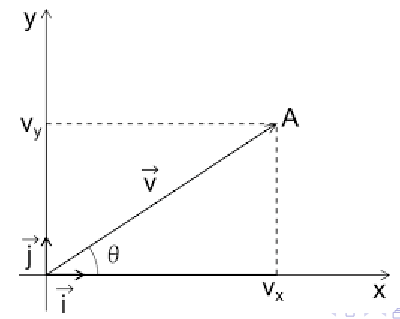
\includegraphics[width=\textwidth]{images/D2.png}
        \label{fig:Trend_Seasonality}
    \end{minipage}
    \hfill
    \begin{minipage}{0.4\textwidth}
        \centering
        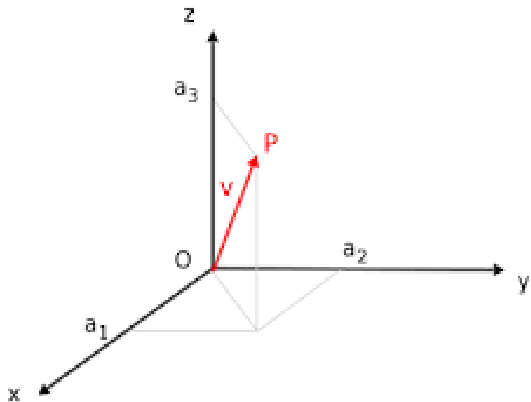
\includegraphics[width=\textwidth]{images/D3.png}
        \label{fig:Residuals}
    \end{minipage}
    \label{fig:TS_Residuals}
\end{figure}

\begin{wrapfigure}{r}{0.4\textwidth}
    \centering
    \vspace{-10pt}
    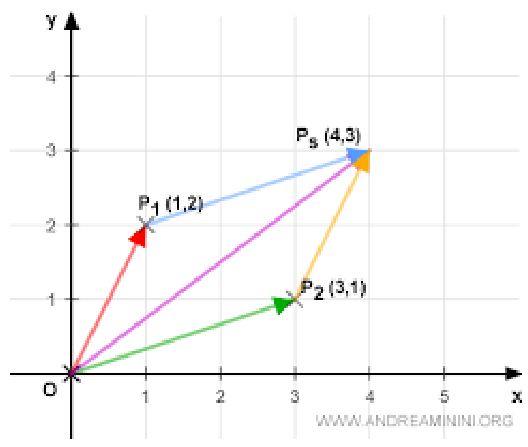
\includegraphics[width=\linewidth]{images/PA.png}
    \label{fig:Scaled Dot Product Attention}
    \vspace{-10pt}
\end{wrapfigure}
Sui vettori (o sui punti) si può definire un’\textbf{operazione di somma}.  
Siano:
\[
\mathbf{v} = (x_1, x_2, \ldots, x_n), \quad \mathbf{w} = (y_1, y_2, \ldots, y_n)
\]

La loro somma è data da:
\[
\mathbf{v} + \mathbf{w} = (x_1 + y_1, \; x_2 + y_2, \; \ldots, \; x_n + y_n)
\]
Questa operazione corrisponde graficamente all’applicazione della regola del parallelogramma.


\subsection{Prodotto per scalari}

Si può definire anche un’operazione di \textbf{prodotto per scalari}.  
In particolare, se 
\[
\mathbf{v} = (x_1, x_2, \ldots, x_n) \quad \text{e} \quad \lambda \in \mathbb{R},
\]
allora
\[
\lambda \mathbf{v} = (\lambda x_1, \lambda x_2, \ldots, \lambda x_n).
\]

Questa operazione equivale a \textbf{dilatare} (o \textbf{contrarre} se $\lambda < 1$) il vettore $\mathbf{v}$ di un fattore $\lambda$.  
Se $\lambda < 0$, \textbf{cambia anche il verso} del vettore.

Lo spazio $(\mathbb{R}^n, +, \cdot)$ si dice \textbf{spazio vettoriale}.  

\[
\mathbf{0} = (0, 0, \ldots, 0)
\]
è l’\textbf{elemento neutro} o \textbf{vettore nullo}.

\[
-\mathbf{v} = (-x_1, -x_2, \ldots, -x_n)
\]
è l’\textbf{opposto} di $\mathbf{v}$.

\subsection{Base canonica di $\mathbb{R}^n$}

In $\mathbb{R}^n$ ogni vettore può essere scritto come \textbf{combinazione lineare} di $n$ particolari vettori detti \textbf{base canonica di} $\mathbb{R}^n$.

Tali vettori si indicano con $\hat{e}_k$, $k = 1, \ldots, n$:
\[
\hat{e}_1 = (1, 0, 0, \ldots, 0), \quad 
\hat{e}_2 = (0, 1, 0, \ldots, 0), \quad 
\ldots, \quad 
\hat{e}_n = (0, 0, 0, \ldots, 1)
\]

Un qualunque vettore $\forall \mathbf{v} \in \mathbb{R}^n$, con 
\[
\mathbf{v} = (x_1, x_2, \ldots, x_n),
\]
si può scrivere come:
\[
\mathbf{v} = \sum_{i=1}^{n} x_i \hat{e}_i = 
x_1 \hat{e}_1 + x_2 \hat{e}_2 + \cdots + x_n \hat{e}_n =
x_1(1, 0, \ldots, 0) + \cdots + x_n(0, 0, \ldots, 1).
\]

\subsection{Modulo o norma di un vettore}

Il \textbf{modulo} (o \textbf{norma}) di un vettore rappresenta la sua lunghezza; se visto come punto, è la \textbf{distanza dall’origine}.

Sia $\mathbf{v} = (x_1, x_2, \ldots, x_n)$:
\[
|\mathbf{v}| = \sqrt{x_1^2 + x_2^2 + \cdots + x_n^2}
\]

\textbf{Proprietà del modulo:}
\begin{enumerate}
    \item $\forall \mathbf{v} \in \mathbb{R}^n$, $|\mathbf{v}| \ge 0$ e $|\mathbf{v}| = 0 \Leftrightarrow \mathbf{v} = \mathbf{0}$;
    \item $\forall \mathbf{v} \in \mathbb{R}^n$, $\forall \lambda \in \mathbb{R}$, $|\lambda \mathbf{v}| = |\lambda| \cdot |\mathbf{v}|$;
    \item $\forall \mathbf{v}_1, \mathbf{v}_2 \in \mathbb{R}^n$, 
    \[
    |\mathbf{v}_1 + \mathbf{v}_2| \leq |\mathbf{v}_1| + |\mathbf{v}_2|
    \]
    (detta \textbf{disuguaglianza triangolare}).
\end{enumerate}

\subsection{Distanza tra vettori}

Con il modulo si può definire una \textbf{distanza} tra vettori (o punti) di $\mathbb{R}^n$.

Se 
\[
\mathbf{v} = (x_1, x_2, \ldots, x_n), \quad 
\mathbf{w} = (y_1, y_2, \ldots, y_n),
\]
allora
\[
|\mathbf{v} - \mathbf{w}| = \sqrt{(x_1 - y_1)^2 + (x_2 - y_2)^2 + \cdots + (x_n - y_n)^2}.
\]

La distanza tra $\mathbf{v}$ e $\mathbf{w}$ è la \textbf{lunghezza del segmento congiungente} i due punti.

\subsection{Prodotto scalare}

Un’altra operazione fondamentale tra vettori è il \textbf{prodotto scalare}, che associa a due vettori un numero reale.

Dati
\[
\mathbf{v} = (x_1, x_2, \ldots, x_n), \quad 
\mathbf{w} = (y_1, y_2, \ldots, y_n),
\]
si definisce:
\[
\langle \mathbf{v}, \mathbf{w} \rangle = \mathbf{v} \cdot \mathbf{w} = x_1 y_1 + x_2 y_2 + \cdots + x_n y_n = \sum_{i=1}^{n} x_i y_i.
\]

\textbf{Osservazione:}
\[
\mathbf{v} \cdot \mathbf{w} = |\mathbf{v}| \, |\mathbf{w}| \, \cos(\theta)
\]
dove $\theta$ è l’angolo compreso tra $\mathbf{v}$ e $\mathbf{w}$.

Da qui segue che:
\[
\langle \mathbf{v}, \mathbf{w} \rangle = 0 \iff \mathbf{v}, \mathbf{w} \text{ sono ortogonali}.
\]

\textbf{Proprietà del prodotto scalare:}
\begin{enumerate}
    \item $\forall \mathbf{v}, \mathbf{w} \in \mathbb{R}^n$, $\langle \mathbf{v}, \mathbf{w} \rangle = \langle \mathbf{w}, \mathbf{v} \rangle$;
    \item $\forall \mathbf{v}, \mathbf{w}_1, \mathbf{w}_2 \in \mathbb{R}^n$, 
    \[
    \langle \mathbf{v}, \mathbf{w}_1 + \mathbf{w}_2 \rangle = \langle \mathbf{v}, \mathbf{w}_1 \rangle + \langle \mathbf{v}, \mathbf{w}_2 \rangle;
    \]
    \item $\forall \mathbf{v}, \mathbf{w} \in \mathbb{R}^n$, $\forall \lambda \in \mathbb{R}$,
    \[
    \langle \lambda \mathbf{v}, \mathbf{w} \rangle = \langle \mathbf{v}, \lambda \mathbf{w} \rangle = \lambda \langle \mathbf{v}, \mathbf{w} \rangle;
    \]
    \item $\forall \mathbf{v}, \mathbf{w} \in \mathbb{R}^n$, 
    \[
    |\langle \mathbf{v}, \mathbf{w} \rangle| \leq |\mathbf{v}| \cdot |\mathbf{w}|
    \]
    (detta \textbf{disuguaglianza di Cauchy-Schwarz});
    \item $\forall \mathbf{v} \in \mathbb{R}^n$, $\langle \mathbf{v}, \mathbf{v} \rangle = |\mathbf{v}|^2$.
\end{enumerate}


\subsection*{Prodotto vettoriale (in $\mathbb{R}^3$)}

In $\mathbb{R}^3$ si può definire anche il \textbf{prodotto vettoriale} tra due vettori $\mathbf{u}$ e $\mathbf{v}$.

Il risultato è un terzo vettore $\mathbf{w} = \mathbf{u} \times \mathbf{v}$:
\begin{compactitemize}
    \item ortogonale al piano contenente $\mathbf{u}$ e $\mathbf{v}$;
    \item con verso determinato dalla \textbf{regola della mano destra};
    \item con modulo pari all’\textbf{area del parallelogramma} avente per lati $\mathbf{u}$ e $\mathbf{v}$.
\end{compactitemize}

\[
|\mathbf{w}| = |\mathbf{u}| \, |\mathbf{v}| \, |\sin(\theta)|
\]

\textbf{Attenzione:} il prodotto vettoriale non è commutativo:
\[
\mathbf{u} \times \mathbf{v} = -(\mathbf{v} \times \mathbf{u}).
\]

\section{Richiami di algebra e analisi multivariata}
\subsection{Varietà affine}
\begin{wrapfigure}{r}{0.4\textwidth}
    \centering
    \vspace{-10pt}
    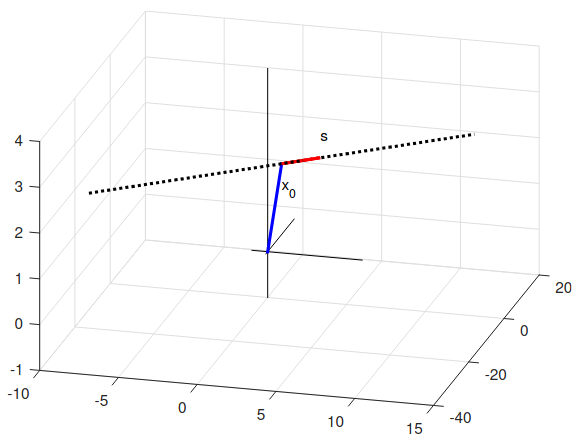
\includegraphics[width=\linewidth]{images/VA.png}
    \label{fig:Scaled Dot Product Attention}
    \vspace{-10pt}
\end{wrapfigure}
Dato un vettore $s \in R^n$, si dice \textbf{varietà affine} di $R^n$ passante per $x_0 \in R^n$ la traslazione del sottospazio
generato da s in $x_0$:
\[
    x(\alpha)= x_0 + \alpha*s , \alpha \in R^n
\]
Al variare di $\alpha , x(\alpha) $ individua una retta nello spazio

\subsection{Derivata direzionale unilaterale}
Sia $f : \mathbb{R}^n \to \mathbb{R}$ e $x_0 \in \mathbb{R}^n$.

Si dice \textbf{derivata direzionale unilaterale} di $f$ rispetto alla direzione $\mathbf{s}$ in $x_0$ il seguente limite (se esiste, può anche essere $\pm \infty$):

\[
f'(x_0; \mathbf{s}) = \lim_{\alpha \to 0^+} \frac{f(x_0 + \alpha \mathbf{s}) - f(x_0)}{\alpha}
\]

Si osserva che:
\[
- f'(x_0; -\mathbf{s}) = \lim_{\alpha \to 0^-} \frac{f(x_0 + \alpha \mathbf{s}) - f(x_0)}{\alpha}
\]

Se \textbf{entrambi i limiti esistono finiti e sono uguali}, allora la funzione $f$ ha \textbf{derivata direzionale} rispetto a $\mathbf{s}$ in $x_0$, e si ha:

\[
\frac{d f(x_0; \mathbf{s})}{d \alpha} = f'(x_0; \mathbf{s}) = -f'(x_0; -\mathbf{s})
\]

Se la \textbf{derivata direzionale} esiste per \textbf{ogni direzione} $\mathbf{s}$ in $x_0$, allora $f$ è \textbf{differenziabile in} $x_0$.

In particolare, la \textbf{derivata direzionale} rispetto a un vettore della \textbf{base canonica} $\hat{e}_i$ in $x_0$ (se esiste finita) si chiama \textbf{derivata parziale} e si indica con:
\[
\frac{\partial f(x_0)}{\partial x_i}
\]
cioè la derivata di $f$ rispetto alla $i$-esima variabile in $x_0$.

\subsection{Derivate Parziali}
Sia 
\[
f : \mathbb{R}^n \to \mathbb{R}
\]
una funzione e $x_0 \in \mathbb{R}^n$; sia $\hat{e}_i$, con $i = 1, \ldots, n$, il \textbf{$i$-esimo vettore della base canonica} di $\mathbb{R}^n$.
Se esiste finito il seguente limite:
\[
\lim_{\alpha \to 0} \frac{f(x_0 + \alpha \hat{e}_i) - f(x_0)}{\alpha},
\]
esso viene detto la \textbf{$i$-esima derivata parziale} di $f$ in $x_0$ e si denota con:
\[
\frac{\partial f(x_0)}{\partial x_i}.
\]
Se in $x_0$ esistono le derivate parziali per ogni $i = 1, \ldots, n$, allora il \textbf{vettore colonna} delle derivate parziali si chiama \textbf{gradiente} di $f$ in $x_0$:
\[
\nabla f(x_0) =
\begin{pmatrix}
\dfrac{\partial f(x_0)}{\partial x_1} \\[6pt]
\vdots \\[4pt]
\dfrac{\partial f(x_0)}{\partial x_n}
\end{pmatrix}
\]
In tal caso, si dice che $f$ è \textbf{differenziabile in} $x_0$.

Si dice che $f$ è \textbf{differenziabile} se esiste il gradiente di $f$ per ogni $x \in \mathbb{R}^n$.

Se le derivate parziali sono tutte \textbf{continue} per ogni $x$, allora $f$ si dice \textbf{differenziabile con continuità} o, in forma compatta, $f \in C^1$, cioè $f$ è una \textbf{funzione regolare}.

\subsubsection{Derivate seconde e matrice Hessiana}
Se le derivate parziali di $f$ sono a loro volta tutte funzioni \textbf{differenziabili con continuità}, si denota con:
\[
\frac{\partial^2 f(x)}{\partial x_i \, \partial x_j}
\]
la \textbf{$i$-esima derivata parziale} della derivata parziale $\dfrac{\partial f(x)}{\partial x_j}$.

La \textbf{matrice Hessiana} di $f$ è la matrice quadrata di ordine $n$ il cui $(i,j)$-esimo elemento è $\dfrac{\partial^2 f(x)}{\partial x_i \, \partial x_j}$, e si indica con:
\[
\nabla^2 f(x)
\]

Essa è \textbf{simmetrica}, cioè:
\[
\nabla^2 f(x)^{T} = \nabla^2 f(x)
\]

Esplicitamente:
\[
\nabla^2 f(x) =
\begin{pmatrix}
\dfrac{\partial^2 f(x)}{\partial x_1^2} & \dfrac{\partial^2 f(x)}{\partial x_1 \partial x_2} & \cdots & \dfrac{\partial^2 f(x)}{\partial x_1 \partial x_n} \\[8pt]
\dfrac{\partial^2 f(x)}{\partial x_2 \partial x_1} & \dfrac{\partial^2 f(x)}{\partial x_2^2} & \cdots & \dfrac{\partial^2 f(x)}{\partial x_2 \partial x_n} \\[8pt]
\vdots & \vdots & \ddots & \vdots \\[8pt]
\dfrac{\partial^2 f(x)}{\partial x_n \partial x_1} & \dfrac{\partial^2 f(x)}{\partial x_n \partial x_2} & \cdots & \dfrac{\partial^2 f(x)}{\partial x_n^2}
\end{pmatrix}
\]

\subsubsection{Jacobiana}
Sia 
\[
f : \mathbb{R}^n \to \mathbb{R}^m.
\]

Se le componenti della funzione $f$, ossia $f_1, f_2, \ldots, f_m$, sono \textbf{differenziabili}, allora:
\[
\nabla f(x) = [ \nabla f_1(x) \; \nabla f_2(x) \; \cdots \; \nabla f_m(x) ]
\]
è una \textbf{matrice $n \times m$}.

La trasposta $m \times n$ di tale matrice si dice \textbf{Jacobiana} di $f$ in $x$ e si indica con:
\[
J_f(x) = \nabla f(x)^{T}
\]

Esplicitamente:
\[
J_f(x) =
\begin{pmatrix}
\dfrac{\partial f_1(x)}{\partial x_1} & \dfrac{\partial f_1(x)}{\partial x_2} & \cdots & \dfrac{\partial f_1(x)}{\partial x_n} \\[8pt]
\dfrac{\partial f_2(x)}{\partial x_1} & \dfrac{\partial f_2(x)}{\partial x_2} & \cdots & \dfrac{\partial f_2(x)}{\partial x_n} \\[8pt]
\vdots & \vdots & \ddots & \vdots \\[8pt]
\dfrac{\partial f_m(x)}{\partial x_1} & \dfrac{\partial f_m(x)}{\partial x_2} & \cdots & \dfrac{\partial f_m(x)}{\partial x_n}
\end{pmatrix}
\]

\subsubsection{Regola pratica per la derivata direzionale}
Sia 
\[
f : \mathbb{R}^n \to \mathbb{R}
\]
una funzione \textbf{differenziabile} e $x_0 \in \mathbb{R}^n$.

Ricordando che 
\[
x(\alpha) = x_0 + \alpha \mathbf{s},
\]
per la \textbf{regola di concatenamento delle funzioni composte} vale:

\[
\frac{d\,\cdot}{d\alpha} = \sum_{i=1}^{n} \frac{\partial\,\cdot}{\partial x_i} \frac{d x_i(\alpha)}{d\alpha}
\]

Poiché $\dfrac{d x_i(\alpha)}{d\alpha} = s_i$, otteniamo:

\[
\frac{d\,\cdot}{d\alpha} = \sum_{i=1}^{n} s_i \frac{\partial\,\cdot}{\partial x_i} = \mathbf{s}^T \nabla (\cdot) = \nabla(\cdot)^T \mathbf{s}.
\]

Applicando questa regola alla funzione composta $f(x(\alpha)) = f \circ x(\alpha)$, si ottiene:

\[
\frac{d f(x(\alpha))}{d\alpha} = \mathbf{s}^T \nabla f(x(\alpha)) = \mathbf{s}^T \mathbf{g} = \mathbf{g}^T \mathbf{s},
\]
dove 
\[
\mathbf{g} = \mathbf{g}(x(\alpha)) = \nabla f(x(\alpha)).
\]

Questa derivata rappresenta \textbf{l’inclinazione} o \textbf{la variazione di} $f$ \textbf{lungo la direzione} $\mathbf{s}$ in $x(\alpha)$.

Assumendo che $f$ sia \textbf{differenziabile con continuità}, è possibile calcolare la \textbf{derivata seconda} di $f$ rispetto ad $\alpha$ in $x(\alpha)$:

\[
\frac{d^2 f(x(\alpha))}{d\alpha^2}
= \frac{d}{d\alpha} \left( \frac{d f(x(\alpha))}{d\alpha} \right)
= \mathbf{s}^T \nabla \big( \nabla f(x(\alpha))^T \mathbf{s} \big)
= \mathbf{s}^T \nabla^2 f(x(\alpha)) \, \mathbf{s}
= \mathbf{s}^T H \mathbf{s},
\]
dove 
\[
H = H(x(\alpha)) = \nabla^2 f(x(\alpha))
\]
è la \textbf{matrice Hessiana} di $f$ in $x(\alpha)$.

Il termine 
\[
\mathbf{s}^T H \mathbf{s}
\]
rappresenta la \textbf{curvatura di} $f$ \textbf{lungo la direzione} $\mathbf{s}$ in $x(\alpha)$.

La dipendenza della curvatura (e della derivata direzionale) dalla \textbf{lunghezza del vettore direzione} $\mathbf{s}$ può essere eliminata considerando il \textbf{versore associato}:
\[
\hat{\mathbf{s}} = \frac{\mathbf{s}}{\|\mathbf{s}\|},
\]
oppure imponendo direttamente che $\|\mathbf{s}\| = 1$.

In tal caso, $\hat{\mathbf{s}}$ indica la \textbf{direzione pura} senza influenza della scala, e le quantità:
\[
\frac{d f(x(\alpha))}{d\alpha} = \hat{\mathbf{s}}^T \nabla f(x(\alpha))
\quad \text{e} \quad
\frac{d^2 f(x(\alpha))}{d\alpha^2} = \hat{\mathbf{s}}^T \nabla^2 f(x(\alpha)) \, \hat{\mathbf{s}}
\]
descrivono rispettivamente \textbf{l’inclinazione} e la \textbf{curvatura normalizzata} di $f$ lungo la direzione $\hat{\mathbf{s}}$.

\subsection{Curve di livello}
Data la costante $c \in \mathbb{R}$, si dice \emph{curva di livello} di $f$ associata a $c$ l’insieme
\[
L_c(f) = \{x \in \mathbb{R}^n : f(x) = c\}.
\]
L’\emph{insieme di livello} di $f$ associato a $c$ è definito come
\[
L_{\leq c}(f) = \{x \in \mathbb{R}^n : f(x) \leq c\}.
\]
\noindent\textbf{Osservazioni}:
\begin{itemize}
    \item I vettori $\pm \dfrac{\nabla f(x_0)}{\|\nabla f(x_0)\|}$ sono direzioni ortogonali alla curva di livello di $f$ in $x_0$, o meglio alla tangente alla curva di livello di $f$ in $x_0$; infatti, detta $t$ la direzione della varietà affine per $x_0$ (iperpiano) tangente alla curva di livello $L_{f(x_0)}(f)$, si ha che $0 = \dfrac{df(x_0)}{d\alpha} = \nabla f(x_0)^T t$, ossia $t$ e $\nabla f(x_0)$ sono ortogonali.
    
    \item I vettori $\pm \dfrac{\nabla f(x_0)}{\|\nabla f(x_0)\|}$ sono la direzione di massima crescita e di massima decrescita di $f$ in $x_0$; infatti, fra tutti i versori $s$, se $\varphi$ è l’angolo tra $s$ e $\nabla f(x_0)$, il versore per cui si ha la massima inclinazione di $f$, ossia $\dfrac{df(x_0)}{d\alpha}$ massima o minima,
    \[
    \dfrac{df(x_0)}{d\alpha} = \nabla f(x_0)^T s = \|\nabla f(x_0)\| \|s\| \cos(\varphi),
    \]
    è il vettore per cui $\cos(\varphi) = \pm 1$, ossia $\varphi = 0, \pi$, cioè $s = \pm \dfrac{\nabla f(x_0)}{\|\nabla f(x_0)\|}$.
\end{itemize}

\section{Funzione obiettivo lineare}
Sia $\ell : \mathbb{R}^n \to \mathbb{R}$ una funzione lineare:
\[
\ell(x) = a^T x + b = \sum_{i=1}^{n} a_i x_i + b
\]
con $a \in \mathbb{R}^n$ e $b \in \mathbb{R}$ costanti.
\noindent Vale la regola di derivazione del prodotto:
\[
\nabla(u^T v) = (\nabla u^T)v + (\nabla v^T)u.
\]
Per ogni $i = 1, \ldots, n$, data la funzione $x \mapsto x_i$, si ha che $\nabla x_i = e_i$, cosicché
\[
\nabla x^T = \nabla(x_1, x_2, \ldots, x_n) = [e_1 \ e_2 \ \ldots \ e_n] = I_n.
\]
\noindent È immediato verificare che
\[
\nabla \ell(x) = (\nabla a^T)x + \nabla x^T a = I_n \cdot a = a,
\]
dalla regola
\[
\nabla \ell(x) = \sum_{i=1}^{n} \frac{\partial \ell}{\partial x_i} \nabla x_i = \sum_{i=1}^{n} a_i e_i = a.
\]
\noindent Per la derivazione di funzione composta, si ha infine
\[
\nabla^2 \ell(x) = 0_n.
\]
